% Practice Test 07 — Virginia Edition
% Questions: 30 (18 MC + 12 SA)
% Generated by scripts/generate_practice_tests.py

\begin{practiceQuestion}{1-4-q23}{sa}
\begin{questionText}
The equation $d = 45t$ gives distance in miles for time in hours. How far does the car travel in $2\frac{1}{2}$ hours?
\end{questionText}
\correctAnswer{$112.5$ miles}
\explanation{$d = 45 \times 2.5 = 112.5$ miles.}
\end{practiceQuestion}

\begin{practiceQuestion}{2-1-q09}{mc}
\begin{questionText}
A student answered $35$ out of $50$ questions correctly. What percent did the student get right?
\end{questionText}
\choiceA{$35\%$}
\choiceB{$50\%$}
\choiceC{$65\%$}
\choiceD{$70\%$}
\correctAnswer{D}
\explanation{Divide the part by the whole: $35 \div 50 = 0.70 = 70\%$.}
\end{practiceQuestion}

\begin{practiceQuestion}{2-2-q29}{gsa}
\begin{questionText}
The double number line below shows a percent relationship. What number goes at the question mark?

\begin{center}
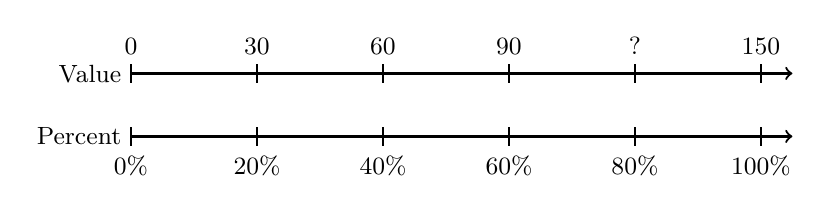
\begin{tikzpicture}[scale=0.8]
  % Top number line (values)
  \draw[thick,->] (0,1) -- (10.5,1);
  \node[left,font=\small] at (0,1) {Value};
  \foreach \x/\lab in {0/0, 2/30, 4/60, 6/90, 8/?, 10/150} {
    \draw[thick] (\x,0.85) -- (\x,1.15);
    \node[above,font=\small] at (\x,1.15) {\lab};
  }
  % Bottom number line (percent)
  \draw[thick,->] (0,0) -- (10.5,0);
  \node[left,font=\small] at (0,0) {Percent};
  \foreach \x/\lab in {0/0\%, 2/20\%, 4/40\%, 6/60\%, 8/80\%, 10/100\%} {
    \draw[thick] (\x,-0.15) -- (\x,0.15);
    \node[below,font=\small] at (\x,-0.15) {\lab};
  }
\end{tikzpicture}
\end{center}
\end{questionText}
\correctAnswer{$120$}
\explanation{The whole ($100\%$) corresponds to $150$. At $80\%$: $\frac{n}{150} = \frac{80}{100}$ → $n = 120$.}
\end{practiceQuestion}

\begin{practiceQuestion}{2-3-q27}{gmc}
\begin{questionText}
The double number line shows an original price and a discounted price. What is the percent decrease?

\begin{center}
\begin{tikzpicture}[scale=0.7]
  % Top: price
  \draw[thick,->] (0,1) -- (10.5,1);
  \node[left,font=\small] at (0,1) {Price};
  \draw[thick] (0,0.85) -- (0,1.15); \node[above,font=\small] at (0,1.15) {$\$0$};
  \draw[thick] (6,0.85) -- (6,1.15); \node[above,font=\small] at (6,1.15) {$\$48$};
  \draw[thick] (10,0.85) -- (10,1.15); \node[above,font=\small] at (10,1.15) {$\$80$};
  % Bottom: percent
  \draw[thick,->] (0,0) -- (10.5,0);
  \node[left,font=\small] at (0,0) {\%};
  \draw[thick] (0,-0.15) -- (0,0.15); \node[below,font=\small] at (0,-0.15) {$0\%$};
  \draw[thick] (6,-0.15) -- (6,0.15); \node[below,font=\small] at (6,-0.15) {?};
  \draw[thick] (10,-0.15) -- (10,0.15); \node[below,font=\small] at (10,-0.15) {$100\%$};
  % Arrow showing decrease
  \draw[thick,->,funRed] (10,1.6) to[bend left=20] node[above,font=\small]{discount} (6,1.6);
\end{tikzpicture}
\end{center}
\end{questionText}
\choiceA{$32\%$}
\choiceB{$40\%$}
\choiceC{$48\%$}
\choiceD{$60\%$}
\correctAnswer{B}
\explanation{The sale price $\$48$ is $\frac{48}{80} = 60\%$ of the original. The percent decrease is $100\% - 60\% = 40\%$.}
\end{practiceQuestion}

\begin{practiceQuestion}{2-7-q19}{sa}
\begin{questionText}
You estimated a room is $18$ feet long. The actual length is $20$ feet. What is the percent error?
\end{questionText}
\correctAnswer{$10\%$}
\explanation{$\frac{|18 - 20|}{20} \times 100 = \frac{2}{20} \times 100 = 10\%$.}
\end{practiceQuestion}

\begin{practiceQuestion}{3-2-q21}{sa}
\begin{questionText}
A hiker starts at an elevation of $-30$ feet (below sea level). She climbs $45$ feet. What is her new elevation?
\end{questionText}
\correctAnswer{$15$ feet}
\explanation{$(-30) + 45 = 15$. She is now $15$ feet above sea level.}
\end{practiceQuestion}

\begin{practiceQuestion}{3-3-q12}{mc}
\begin{questionText}
What is $(-3) - 5 - (-10)$?
\end{questionText}
\choiceA{$-18$}
\choiceB{$2$}
\choiceC{$-2$}
\choiceD{$12$}
\correctAnswer{B}
\explanation{Rewrite: $(-3) + (-5) + 10$. Add negatives: $-3 + (-5) = -8$. Then $-8 + 10 = 2$.}
\end{practiceQuestion}

\begin{practiceQuestion}{3-4-q04}{mc}
\begin{questionText}
What is $-\dfrac{2}{3} - \dfrac{1}{6}$?
\end{questionText}
\choiceA{$-\dfrac{1}{6}$}
\choiceB{$-\dfrac{5}{6}$}
\choiceC{$\dfrac{5}{6}$}
\choiceD{$-\dfrac{1}{2}$}
\correctAnswer{B}
\explanation{Rewrite subtraction: $-\frac{2}{3} + (-\frac{1}{6})$. Common denominator $6$: $-\frac{4}{6} + (-\frac{1}{6}) = -\frac{5}{6}$.}
\end{practiceQuestion}

\begin{practiceQuestion}{4-3-q16}{mc}
\begin{questionText}
Expand and simplify $2(4n - 3) - (n + 1)$.
\end{questionText}
\choiceA{$7n - 7$}
\choiceB{$9n - 7$}
\choiceC{$7n - 5$}
\choiceD{$9n - 4$}
\correctAnswer{A}
\explanation{Expand: $8n - 6 - n - 1$. Combine: $(8n - n) + (-6 - 1) = 7n - 7$.}
\end{practiceQuestion}

\begin{practiceQuestion}{4-4-q08}{mc}
\begin{questionText}
Factor $24x - 16$.
\end{questionText}
\choiceA{$4(6x - 4)$}
\choiceB{$8(3x - 2)$}
\choiceC{$2(12x - 8)$}
\choiceD{$6(4x - 2)$}
\correctAnswer{B}
\explanation{GCF of $24$ and $16$ is $8$. Factor: $24x \div 8 = 3x$ and $-16 \div 8 = -2$. Result: $8(3x - 2)$.}
\end{practiceQuestion}

\begin{practiceQuestion}{5-4-q13}{mc}
\begin{questionText}
A shirt is on sale for $\dfrac{2}{3}$ of its original price. After using a $\$5$ coupon, you pay $\$15$. What equation finds the original price $p$?
\end{questionText}
\choiceA{$\dfrac{2}{3}p + 5 = 15$}
\choiceB{$p - \dfrac{2}{3} - 5 = 15$}
\choiceC{$\dfrac{2}{3}p - 5 = 15$}
\choiceD{$\dfrac{2}{3}(p - 5) = 15$}
\correctAnswer{C}
\explanation{Sale price is $\frac{2}{3}p$. After the $\$5$ coupon: $\frac{2}{3}p - 5 = 15$.}
\end{practiceQuestion}

\begin{practiceQuestion}{5-5-q17}{mc}
\begin{questionText}
Which inequality means ``no more than $25$''?
\end{questionText}
\choiceA{$x > 25$}
\choiceB{$x \geq 25$}
\choiceC{$x < 25$}
\choiceD{$x \leq 25$}
\correctAnswer{D}
\explanation{``No more than $25$'' means $25$ or fewer: $x \leq 25$.}
\end{practiceQuestion}

\begin{practiceQuestion}{5-6-q20}{sa}
\begin{questionText}
Solve $-5x + 15 \geq 30$. Describe the graph.
\end{questionText}
\correctAnswer{$x \leq -3$; closed circle at $-3$, shade left}
\explanation{Subtract $15$: $-5x \geq 15$. Divide by $-5$ and flip: $x \leq -3$. Closed circle at $-3$, shade left.}
\end{practiceQuestion}

\begin{practiceQuestion}{6-1-q26}{gmc}
\begin{questionText}
A blueprint of a house is shown below. The scale is $1$ cm $= 5$ m. What is the actual length of the living room?

\begin{center}
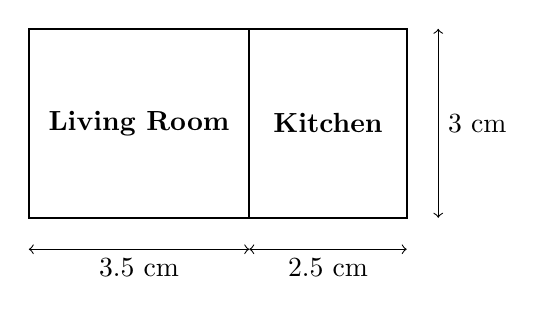
\begin{tikzpicture}[scale=0.8]
  \draw[thick] (0,0) rectangle (6,3);
  \draw[thick] (3.5,0) -- (3.5,3);
  \node at (1.75,1.5) {\textbf{Living Room}};
  \node at (4.75,1.5) {\textbf{Kitchen}};
  \draw[<->] (0,-0.5) -- (3.5,-0.5);
  \node[below] at (1.75,-0.5) {$3.5$ cm};
  \draw[<->] (3.5,-0.5) -- (6,-0.5);
  \node[below] at (4.75,-0.5) {$2.5$ cm};
  \draw[<->] (6.5,0) -- (6.5,3);
  \node[right] at (6.5,1.5) {$3$ cm};
\end{tikzpicture}
\end{center}
\end{questionText}
\choiceA{$3.5$ m}
\choiceB{$12.5$ m}
\choiceC{$15$ m}
\choiceD{$17.5$ m}
\correctAnswer{D}
\explanation{The living room is $3.5$ cm on the drawing. Actual length: $3.5 \times 5 = 17.5$ m.}
\end{practiceQuestion}

\begin{practiceQuestion}{6-2-q29}{gsa}
\begin{questionText}
The rectangle below is drawn at scale $1$ cm $= 8$ m. Redraw it at scale $1$ cm $= 4$ m. What are the new dimensions, and what is the new drawing's area?

\begin{center}
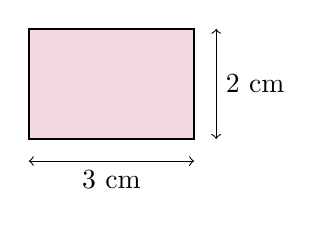
\begin{tikzpicture}[scale=0.7]
  \draw[thick,fill=purple!15] (0,0) rectangle (3,2);
  \draw[<->] (0,-0.4) -- (3,-0.4);
  \node[below] at (1.5,-0.4) {$3$ cm};
  \draw[<->] (3.4,0) -- (3.4,2);
  \node[right] at (3.4,1) {$2$ cm};
\end{tikzpicture}
\end{center}
\end{questionText}
\correctAnswer{$6$ cm by $4$ cm; area $= 24$ cm$^2$}
\explanation{Scale ratio: $\frac{8}{4} = 2$. New dimensions: $3 \times 2 = 6$ cm and $2 \times 2 = 4$ cm. Area: $6 \times 4 = 24$ cm$^2$.}
\end{practiceQuestion}

\begin{practiceQuestion}{6-5-q30}{gsa}
\begin{questionText}
The diagram shows a cube with edge length $6$ cm. A diagonal cut is made from vertex $A$ through the center to the opposite vertex $B$, passing through four faces. What type of shape could this cross-section be?

\begin{center}
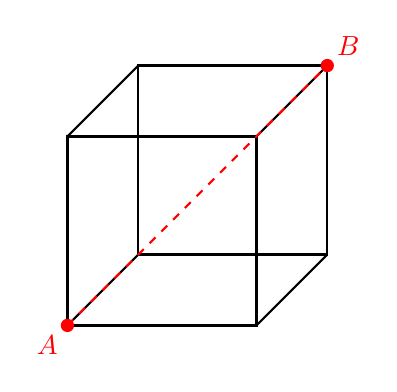
\begin{tikzpicture}[scale=0.6]
  % Front face
  \draw[thick] (0,0) -- (4,0) -- (4,4) -- (0,4) -- cycle;
  % Back face
  \draw[thick] (1.5,1.5) -- (5.5,1.5) -- (5.5,5.5) -- (1.5,5.5) -- cycle;
  % Connecting edges
  \draw[thick] (0,0) -- (1.5,1.5);
  \draw[thick] (4,0) -- (5.5,1.5);
  \draw[thick] (4,4) -- (5.5,5.5);
  \draw[thick] (0,4) -- (1.5,5.5);
  % Diagonal vertices
  \fill[red] (0,0) circle (4pt) node[below left] {$A$};
  \fill[red] (5.5,5.5) circle (4pt) node[above right] {$B$};
  % Diagonal line
  \draw[thick,red,dashed] (0,0) -- (5.5,5.5);
\end{tikzpicture}
\end{center}
\end{questionText}
\correctAnswer{A rectangle}
\explanation{A diagonal cut from one vertex of a cube to the opposite vertex, passing through four faces, creates a rectangular cross-section. The rectangle's dimensions are a face diagonal ($6\sqrt{2}$ cm) by the edge length ($6$ cm).}
\end{practiceQuestion}

\begin{practiceQuestion}{6-6-q24}{sa}
\begin{questionText}
Three angles meet at a point on a line: $50°$, $(2x + 10)°$, and $x°$. Find $x$.
\end{questionText}
\correctAnswer{$40$}
\explanation{Angles on a line sum to $180°$: $50 + 2x + 10 + x = 180$. Combine: $3x + 60 = 180$. Solve: $3x = 120$, $x = 40$.}
\end{practiceQuestion}

\begin{practiceQuestion}{6-7-q19}{sa}
\begin{questionText}
Translate point $N(5, -2)$ left $6$ and up $3$. What are the coordinates of $N'$?
\end{questionText}
\correctAnswer{$N'(-1, 1)$}
\explanation{Left $6$: $5 - 6 = -1$. Up $3$: $-2 + 3 = 1$. So $N'(-1, 1)$.}
\end{practiceQuestion}

\begin{practiceQuestion}{6-8-q13}{mc}
\begin{questionText}
Two similar pentagons have a scale factor of $4$. If a side of the smaller pentagon is $3$ cm, what is the corresponding side of the larger pentagon?
\end{questionText}
\choiceA{$7$ cm}
\choiceB{$12$ cm}
\choiceC{$16$ cm}
\choiceD{$0.75$ cm}
\correctAnswer{B}
\explanation{Larger side $= 3 \times 4 = 12$ cm.}
\end{practiceQuestion}

\begin{practiceQuestion}{7-4-q16}{mc}
\begin{questionText}
A figure is made of a right triangle with legs $6$ cm and $8$ cm, and a rectangle $8$ cm by $3$ cm. What is the total area?
\end{questionText}
\choiceA{$24$ cm$^2$}
\choiceB{$48$ cm$^2$}
\choiceC{$36$ cm$^2$}
\choiceD{$72$ cm$^2$}
\correctAnswer{B}
\explanation{Triangle: $\frac{1}{2} \times 6 \times 8 = 24$ cm$^2$. Rectangle: $8 \times 3 = 24$ cm$^2$. Total: $24 + 24 = 48$ cm$^2$.}
\end{practiceQuestion}

\begin{practiceQuestion}{7-5-q09}{mc}
\begin{questionText}
A rectangular prism has dimensions $7$ m by $4$ m by $3$ m. What is the area of the largest face?
\end{questionText}
\choiceA{$12$ m$^2$}
\choiceB{$21$ m$^2$}
\choiceC{$28$ m$^2$}
\choiceD{$84$ m$^2$}
\correctAnswer{C}
\explanation{The three pairs of faces have areas $7 \times 4 = 28$, $7 \times 3 = 21$, and $4 \times 3 = 12$ m$^2$. The largest is $28$ m$^2$.}
\end{practiceQuestion}

\begin{practiceQuestion}{7-6-q12}{mc}
\begin{questionText}
A pool is $10$ m long, $5$ m wide, and $2$ m deep. How many cubic meters of water does it hold when full?
\end{questionText}
\choiceA{$17$ m$^3$}
\choiceB{$50$ m$^3$}
\choiceC{$100$ m$^3$}
\choiceD{$200$ m$^3$}
\correctAnswer{C}
\explanation{$V = 10 \times 5 \times 2 = 100$ m$^3$.}
\end{practiceQuestion}

\begin{practiceQuestion}{7-7-q08}{mc}
\begin{questionText}
A cylindrical water tank has a radius of $2$ m and a height of $5$ m. How many cubic meters of water can it hold? Use $\pi \approx 3.14$.
\end{questionText}
\choiceA{$31.4$ m$^3$}
\choiceB{$62.8$ m$^3$}
\choiceC{$125.6$ m$^3$}
\choiceD{$20$ m$^3$}
\correctAnswer{B}
\explanation{$V = \pi r^2 h = 3.14 \times 4 \times 5 = 62.8$ m$^3$.}
\end{practiceQuestion}

\begin{practiceQuestion}{8-1-q26}{gmc}
\begin{questionText}
A student surveyed $50$ classmates about their favorite fruit. The results are shown in the bar graph below.

\begin{center}
\begin{tikzpicture}[scale=0.7]
  \draw[thick,->] (0,0) -- (0,6.5) node[above]{\small Number of Students};
  \draw[thick,->] (0,0) -- (8.5,0);
  % bars
  \fill[funBlue!70] (0.5,0) rectangle (1.5,4);
  \fill[funGreen!70] (2.5,0) rectangle (3.5,3);
  \fill[funOrange!70] (4.5,0) rectangle (5.5,2);
  \fill[funRed!70] (6.5,0) rectangle (7.5,1);
  % labels
  \node[below] at (1,0) {\small Apple};
  \node[below] at (3,0) {\small Banana};
  \node[below] at (5,0) {\small Orange};
  \node[below] at (7,0) {\small Grape};
  % y-axis ticks
  \foreach \y in {1,2,3,4,5,6} {
    \draw (-0.1,\y) -- (0.1,\y);
    \node[left] at (0,\y) {\small $\y\times5$};
  }
  % values on bars
  \node[above] at (1,4) {\small $20$};
  \node[above] at (3,3) {\small $15$};
  \node[above] at (5,2) {\small $10$};
  \node[above] at (7,1) {\small $5$};
\end{tikzpicture}
\end{center}

If there are $500$ students in the school, predict how many prefer apples.
\end{questionText}
\choiceA{$20$}
\choiceB{$100$}
\choiceC{$200$}
\choiceD{$250$}
\correctAnswer{C}
\explanation{$\frac{20}{50} = 40\%$ prefer apples. $40\%$ of $500 = 200$.}
\end{practiceQuestion}

\begin{practiceQuestion}{8-3-q13}{mc}
\begin{questionText}
The difference between the means of two groups is $10$. The MAD for each group is $2$. How many MADs apart are the means?
\end{questionText}
\choiceA{$2$}
\choiceB{$5$}
\choiceC{$10$}
\choiceD{$20$}
\correctAnswer{B}
\explanation{$\frac{10}{2} = 5$ MADs apart.}
\end{practiceQuestion}

\begin{practiceQuestion}{8-4-q15}{mc}
\begin{questionText}
Why is it important to use multiple measures (mean, median, range, IQR, MAD) when comparing two groups?
\end{questionText}
\choiceA{One measure tells the complete story}
\choiceB{Using more measures wastes time}
\choiceC{Different measures reveal different aspects of the data}
\choiceD{All measures always give the same conclusion}
\correctAnswer{C}
\explanation{Mean and median show center; range, IQR, and MAD show spread. Together they give a complete picture.}
\end{practiceQuestion}

\begin{practiceQuestion}{8-5-q19}{sa}
\begin{questionText}
Create a stem-and-leaf plot for: $32, 35, 41, 43, 47, 50, 52, 58$. What are the stems?
\end{questionText}
\correctAnswer{Stems: $3, 4, 5$}
\explanation{Stem $3$: leaves $2, 5$. Stem $4$: leaves $1, 3, 7$. Stem $5$: leaves $0, 2, 8$.}
\end{practiceQuestion}

\begin{practiceQuestion}{9-3-q30}{gsa}
\begin{questionText}
The dot plot shows the outcomes of spinning a spinner $40$ times. Each dot represents one spin. How many more times would you need to spin ``B'' to make its experimental probability equal to $\frac{1}{2}$? Assume the total number of spins stays at $40$.

\begin{center}
\begin{tikzpicture}[scale=0.8]
  \draw[thick] (0,0) -- (5,0);
  \node[below,font=\bfseries] at (1,0) {A};
  \node[below,font=\bfseries] at (2.5,0) {B};
  \node[below,font=\bfseries] at (4,0) {C};
  \draw[thick] (1,-0.1) -- (1,0.1);
  \draw[thick] (2.5,-0.1) -- (2.5,0.1);
  \draw[thick] (4,-0.1) -- (4,0.1);
  % A: 15 dots (3 columns of 5)
  \foreach \r in {1,...,5} { \fill[funRed] (0.85,0.2+\r*0.3) circle (0.1); }
  \foreach \r in {1,...,5} { \fill[funRed] (1.15,0.2+\r*0.3) circle (0.1); }
  \foreach \r in {1,...,5} { \fill[funRed] (1.0,0.2+\r*0.3+1.5) circle (0.1); }
  % B: 12 dots (3 columns of 4)
  \foreach \r in {1,...,4} { \fill[funBlue] (2.35,0.2+\r*0.3) circle (0.1); }
  \foreach \r in {1,...,4} { \fill[funBlue] (2.65,0.2+\r*0.3) circle (0.1); }
  \foreach \r in {1,...,4} { \fill[funBlue] (2.5,0.2+\r*0.3+1.2) circle (0.1); }
  % C: 13 dots (3 cols)
  \foreach \r in {1,...,5} { \fill[funGreen] (3.85,0.2+\r*0.3) circle (0.1); }
  \foreach \r in {1,...,5} { \fill[funGreen] (4.15,0.2+\r*0.3) circle (0.1); }
  \foreach \r in {1,...,3} { \fill[funGreen] (4.0,0.2+\r*0.3+1.5) circle (0.1); }
  \node[above,font=\small] at (1,3.5) {$15$};
  \node[above,font=\small] at (2.5,2.8) {$12$};
  \node[above,font=\small] at (4,3.2) {$13$};
\end{tikzpicture}
\end{center}
\end{questionText}
\correctAnswer{$8$}
\explanation{For $P(B) = \frac{1}{2}$, we need $B = \frac{40}{2} = 20$. Currently $B = 12$, so $20 - 12 = 8$ more spins of B are needed (with $8$ fewer from A and C combined).}
\end{practiceQuestion}

\begin{practiceQuestion}{9-6-q06}{mc}
\begin{questionText}
Two dice are rolled. What is the probability that both dice show the same number (doubles)?
\end{questionText}
\choiceA{$\frac{1}{36}$}
\choiceB{$\frac{1}{12}$}
\choiceC{$\frac{1}{6}$}
\choiceD{$\frac{1}{3}$}
\correctAnswer{C}
\explanation{Doubles: $(1,1), (2,2), (3,3), (4,4), (5,5), (6,6)$ — that is $6$ out of $36$. $P = \frac{6}{36} = \frac{1}{6}$.}
\end{practiceQuestion}

\begin{practiceQuestion}{9-7-q25}{sa}
\begin{questionText}
A student runs $200$ simulation trials for an event with theoretical probability $\frac{1}{4}$. They observe the event $54$ times. What is the experimental probability? Is it close to the theoretical value?
\end{questionText}
\correctAnswer{$0.27$; yes, it is close to $0.25$}
\explanation{$P = \frac{54}{200} = 0.27$. Theoretical $= 0.25$. The difference of $0.02$ is small, especially with $200$ trials.}
\end{practiceQuestion}
